\section{Eigene Methoden}
\label{sec:methode}

% --- 2.1 Datensatz ---
\subsection{Datensatz}
\label{subsec:datensatz}

Grundlage der Experimente ist der PatternNet-Datensatz, der speziell für die Evaluation von Verfahren zur Fernerkundungsbildklassifikation und -suche erstellt wurde~\cite{zhou2018patternnet}.
Der Datensatz enthält 30\,400 RGB-Bilder mit einer einheitlichen Bildgröße von $256 \times 256$\,Pixel.
Die Bilder wurden über Google Earth und Google Maps gesammelt und repräsentieren eine Vielzahl von Szenen aus den USA, darunter städtische, ländliche, industrielle und natürliche Umgebungen.
Die Bilder verteilen sich gleichmäßig auf 38 Szenenklassen, wie beispielsweise \textit{airplane}, \textit{bridge}, \textit{forest}, \textit{dense\_residential} und \textit{swimming\_pool}, mit jeweils 800 Bildern pro Klasse.
Die Gleichverteilung der Klassen ist ein Vorteil gegenüber vielen anderen Datensätzen, da keine gesonderte Behandlung von Klassenungleichgewichten erforderlich ist.

Die Aufteilung des Datensatzes in Trainings-, Validierungs- und Testmenge erfolgte stratifiziert, sodass die Klassenverteilung in allen Teilmengen erhalten bleibt.
Es wurde eine Aufteilung von 70\,\% Training, 15\,\% Validierung und 15\,\% Test gewählt.

% --- 2.2 Vorverarbeitung und Augmentation ---
\subsection{Vorverarbeitung und Datenaugmentation}
\label{subsec:augmentation}

Zu Beginn wurde die Anzahl der Bilder pro Klasse auf 100 reduziert, um die Ergebnisse gezielt zu verschlechtern, da die Trainingsergebnisse mit der vollen Anzahl von 800 Bildern pro Klasse bereits sehr gut waren.
Diese künstliche Verknappung der Trainingsdaten führte zu einer deutlichen Verschlechterung der Modellleistung, was die Notwendigkeit vom Einsatz von verschiedenen Techniken zur Verbesserung der Generalisierungsfähigkeit unterstreicht.
Dadurch konnten die Auswirkungen von Augmentationstechniken und Architekturänderungen auf die Leistung besser analysiert werden.

Um die Generalisierungsfähigkeit des Modells zu verbessern und Overfitting entgegenzuwirken, wurden verschiedene Augmentationstechniken auf die Trainingsbilder angewendet.
Diese Transformationen werden zur Laufzeit zufällig auf jedes Bild angewendet, sodass das Netzwerk in jeder Epoche leicht veränderte Varianten der Trainingsbilder sieht.

% TODO: Zoom Hinzufügen
Folgende Augmentationstechniken kamen für die Trainingsmenge zum Einsatz:
\begin{itemize}
    \item \textbf{Zufälliges horizontales Spiegeln}: Das Bild wird mit einer Wahrscheinlichkeit von 50\,\% entlang der horizontalen Achse gespiegelt.
    \item \textbf{Zufälliges vertikales Spiegeln}: Analog dazu wird das Bild mit einer Wahrscheinlichkeit von 50\,\% entlang der vertikalen Achse gespiegelt.
    \item \textbf{Zufällige Rotation}: Das Bild wird um einen zufälligen Winkel im Bereich von $\pm 20^\circ$ gedreht. Da Fernerkundungsbilder keine feste natürliche Orientierung besitzen, ist eine moderate Rotation semantisch sinnvoll und erzeugt gültige neue Trainingsbeispiele.
    \item \textbf{Zufälliges Resizing/Zoom}: Das Bild wird zufällig skaliert, um die Robustheit gegenüber Skalenvariationen zu erhöhen.
\end{itemize}
Für die Validierungs- und Testmenge wurden keine geometrischen Augmentationen angewendet, um eine unverfälschte Bewertung der Modellleistung sicherzustellen.
 
Alle Bilder wurden zunächst in Tensoren konvertiert (Wertebereich $[0, 1]$) und anschließend kanalweise mit einem Mittelwert von $\mu = 0{,}5$ und einer Standardabweichung von $\sigma = 0{,}5$ normalisiert, sodass die resultierenden Pixelwerte im Bereich $[-1, 1]$ liegen.
Diese Normalisierung sorgt für eine zentrierte und skalierte Eingabeverteilung, was die Konvergenz des Trainings begünstigt.

Abbildung~\ref{fig:augmentation} zeigt exemplarisch zwei Grids von je 16~Trainingsbildern nach Anwendung der beschriebenen Augmentationstransformationen.
Die zufälligen Rotationen und Spiegelungen sind an den gedrehten Bildrändern und den schwarzen Eckbereichen erkennbar.
 
\begin{figure}[t]
    \centering
    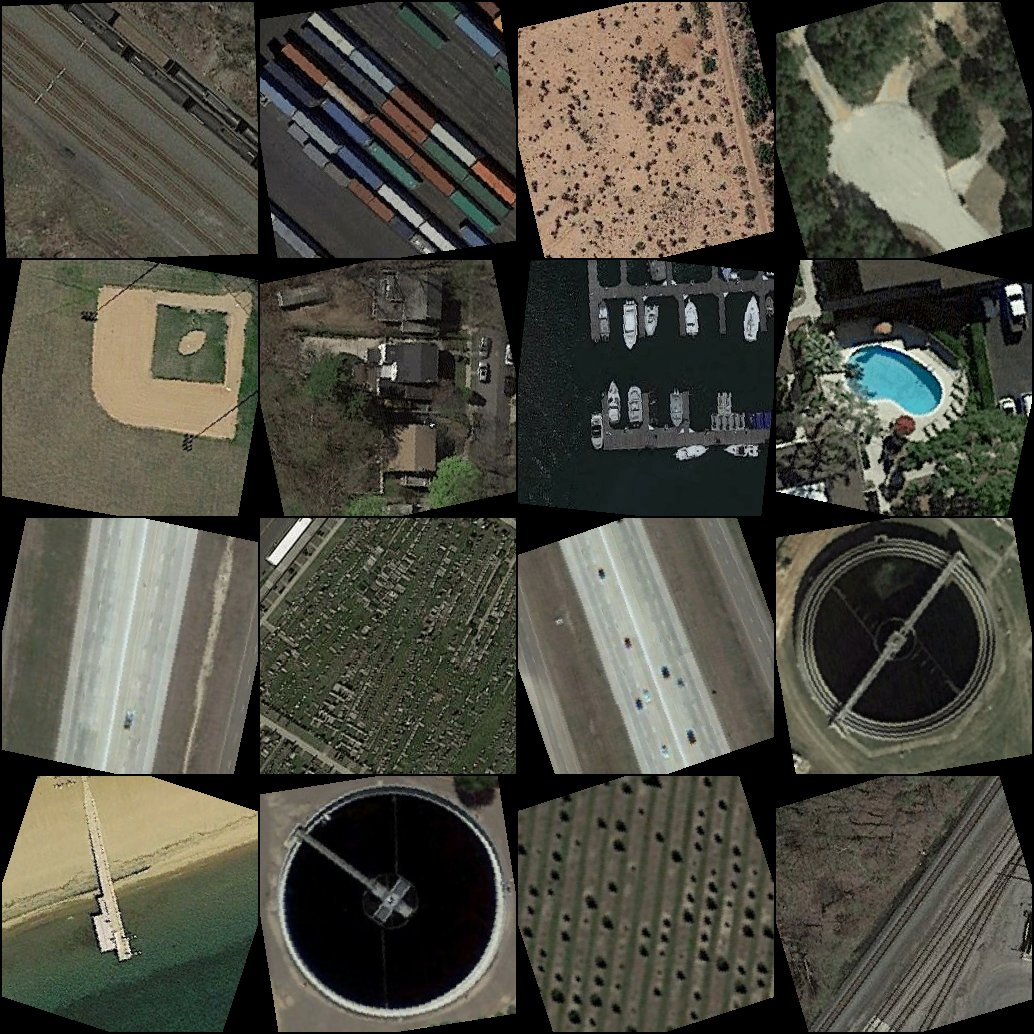
\includegraphics[width=0.48\linewidth]{figures/augmentation_sample_1.png}
    \hfill
    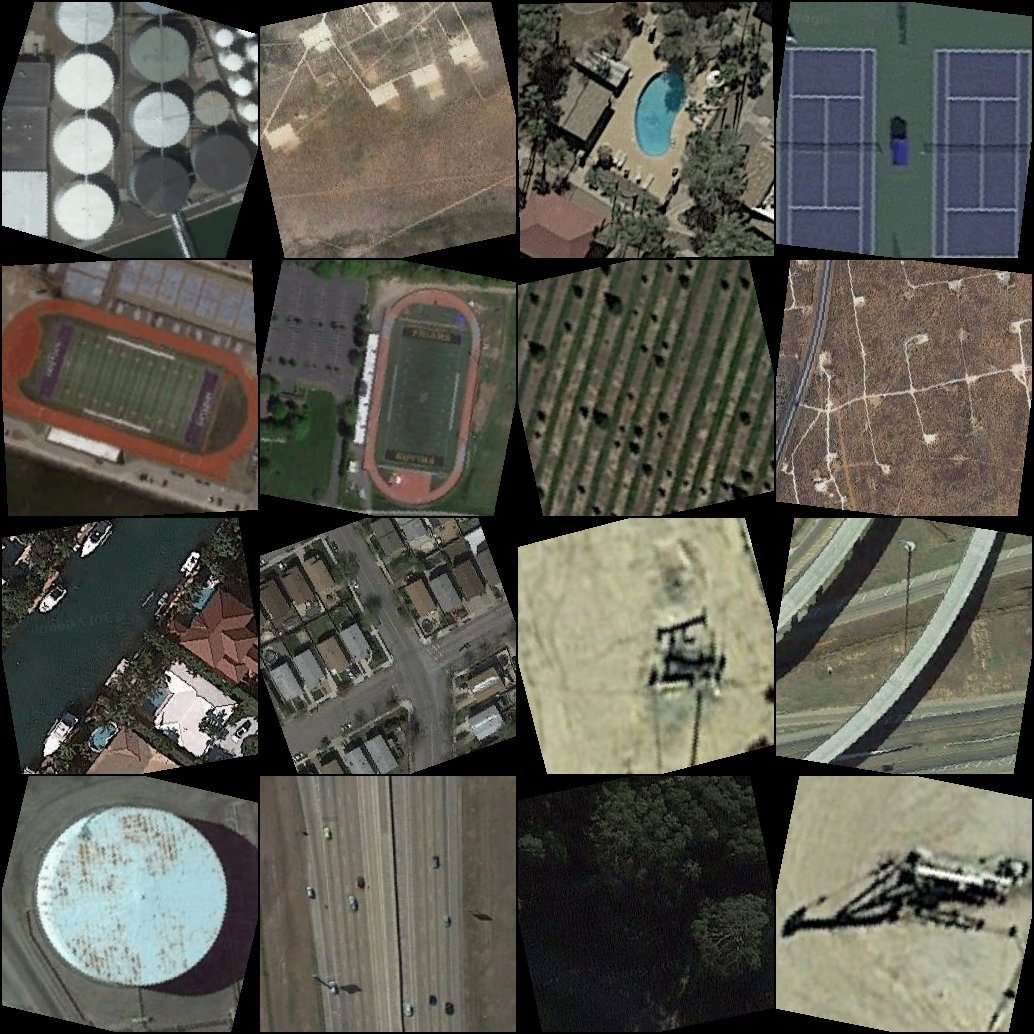
\includegraphics[width=0.48\linewidth]{figures/augmentation_sample_2.png}
    \caption{Beispielhafte Trainingsbilder nach Anwendung der Datenaugmentation (zufälliges horizontales und vertikales Spiegeln, Rotation um bis zu $\pm 20^\circ$) und Normalisierung. Die schwarzen Eckbereiche entstehen durch die zufällige Rotation.}
    \label{fig:augmentation}
\end{figure}

\subsection{Netzarchitektur}
\label{subsec:architektur}
 
Die Entwicklung der Netzarchitektur folgte einem inkrementellen Ansatz: Ausgehend von einem möglichst einfachen Basisnetzwerk wurden schrittweise einzelne Schichtarten oder Techniken hinzugefügt, um deren isolierten Einfluss auf die Klassifikationsleistung zu untersuchen.
Die so gewonnenen Erkenntnisse wurden abschließend in optimierte Gesamtarchitekturen integriert.
Alle Netzwerke verwenden ausschließlich $3 \times 3$-Faltungskerne mit Padding~1, ReLU-Aktivierungsfunktionen sowie Max-Pooling-Schichten ($2 \times 2$, Stride~2) zur räumlichen Reduktion.
Die Ausgabeschicht besteht in jedem Fall aus einer vollständig verbundenen Schicht mit 38~Neuronen (eine pro Klasse), ohne explizite Softmax-Aktivierung, da die verwendete Verlustfunktion \texttt{CrossEntropyLoss} die Softmax-Berechnung intern durchführt.
 
\paragraph{Phase~1: Basisnetzwerk.}
Das \textbf{Base\_Net} bildet den Ausgangspunkt und ist bewusst schlank gehalten.
Es besteht aus fünf Convolution-Layern mit jeweils 32~Feature-Maps (die letzte mit 16~Feature-Maps) und zwei Max-Pooling-Schichten.
Der Klassifikationskopf umfasst drei vollständig verbundene Schichten (16\,384 $\rightarrow$ 128 $\rightarrow$ 128 $\rightarrow$ 38).
Dieses Netzwerk dient als Referenz, um den Effekt jeder einzelnen Änderung bewerten zu können.
 
\paragraph{Phase~2: Isolierte Variation einzelner Komponenten.}
Auf Basis des Base\_Net wurden fünf Varianten erzeugt, die jeweils genau eine Komponente verändern:
 
\begin{itemize}
    \item \textbf{Conv\_Net} -- \textit{Mehr Convolution-Layern}: Die Anzahl der Convolution-Layern wird von fünf auf acht erhöht (alle mit 32~Feature-Maps, letzte mit 16), bei nur zwei Pooling-Schichten. Ziel ist es, den Einfluss einer größeren Netztiefe im Faltungsteil zu untersuchen, ohne die räumliche Auflösung stärker zu reduzieren.
 
    \item \textbf{Dense\_Net} -- \textit{Mehr vollständig verbundene Schichten}: Der Faltungsteil bleibt identisch zum Base\_Net, jedoch wird der Klassifikationskopf auf sieben vollständig verbundene Schichten erweitert (128 $\rightarrow$ 128 $\rightarrow$ 128 $\rightarrow$ 128 $\rightarrow$ 128 $\rightarrow$ 128 $\rightarrow$ 38). Damit wird untersucht, ob ein tieferer Klassifikationskopf die Entscheidungsgrenze verbessert.
 
    \item \textbf{Pooling\_Net} -- \textit{Aggressiveres Downsampling}: Statt zwei werden vier Max-Pooling-Schichten eingesetzt, jeweils nach einer Convolution-Layer. Die räumliche Auflösung wird dadurch auf $16 \times 16$ vor dem Flattening reduziert, was die Parameterzahl im Klassifikationskopf deutlich verringert (4\,096 $\rightarrow$ 128 statt 16\,384 $\rightarrow$ 128).
 
    \item \textbf{Dropout\_Net} -- \textit{Dropout-Regularisierung}: Das Base\_Net wird um eine Dropout-Schicht mit einer Rate von $p = 0{,}5$ zwischen der ersten und zweiten vollständig verbundenen Schicht ergänzt. Damit wird geprüft, ob Dropout das Overfitting reduziert.
 
    \item \textbf{BatchNorm\_Net} -- \textit{Batch-Normalisierung}: Jede Convolution-Layer und die ersten beiden vollständig verbundenen Schichten werden um eine Batch-Normalisierung ergänzt, die vor der ReLU-Aktivierung angewendet wird. Dies soll die Trainingskonvergenz beschleunigen und die Empfindlichkeit gegenüber der Lernrate verringern.
\end{itemize}
 
\paragraph{Phase~3: Kombinierte Architekturen.}
Die Erkenntnisse aus Phase~2 wurden schrittweise in leistungsfähigere Gesamtarchitekturen integriert:
 
\begin{itemize}
    \item \textbf{BatchNorm\_Dense\_Pool\_Net}: Kombiniert die Batch-Normalisierung aus dem BatchNorm\_Net mit drei statt zwei Pooling-Schichten (räumliche Reduktion auf $32 \times 32$). Der Klassifikationskopf umfasst drei vollständig verbundene Schichten mit jeweils vorgeschalteter Batch-Normalisierung (16\,384 $\rightarrow$ 128 $\rightarrow$ 128 $\rightarrow$ 128 $\rightarrow$ 38).
 
    \item \textbf{BatchNorm\_Dense\_Pool\_Conv\_Net}: Erweitert das BatchNorm\_Dense\_Pool\_Net um einen zusätzlichen sechsten Convolution-Layer (32~Filter), ebenfalls mit Batch-Normalisierung.
 
    \item \textbf{BatchNorm\_Dense\_Pool\_Conv\_Dropout\_Net}: Identisch zum BatchNorm\_Dense\_Pool\_Conv\_Net, ergänzt jedoch eine Dropout-Schicht ($p = 0{,}5$) zwischen der zweiten und dritten vollständig verbundenen Schicht. Damit wird Dropout zusätzlich zur Batch-Normalisierung untersucht.
 
    \item \textbf{BatchNorm\_Dense\_Pool\_Conv\_Dropout\_V2\_Net}: Diese Architektur basiert auf dem BatchNorm\_Dense\_Pool\_Conv\_Dropout\_Net, verdoppelt jedoch die Anzahl der Filterkerne in den Convolution-Layern von 32 auf 64 (letzte Schicht: 32 statt 16). Dies erhöht die Kapazität des Netzwerks, mehr parallele Merkmalsrepräsentationen zu lernen, auf Kosten einer größeren Parameterzahl im Faltungsteil.
\end{itemize}
 
Tabelle~\ref{tab:architektur_uebersicht} fasst die wesentlichen Unterschiede der zehn getesteten Architekturen zusammen.
 
% --- 2.4 Trainingsverfahren ---
\subsection{Trainingsverfahren}
\label{subsec:training}
 
Alle Netzwerke wurden unter identischen Bedingungen trainiert, um eine faire Vergleichbarkeit zu gewährleisten.
Als Optimizer diente Adam mit den Standardparametern der PyTorch-Implementierung ($\eta = 10^{-3}$, $\beta_1 = 0{,}9$, $\beta_2 = 0{,}999$).
Ein Learning-Rate-Scheduler wurde nicht eingesetzt, dadurch bleibt die Lernrate über alle Epochen konstant.

Als Verlustfunktion wurde \texttt{CrossEntropyLoss} verwendet, die die Softmax-Berechnung und die negative Log-Likelihood in einem numerisch stabilen Schritt kombiniert und somit die Standardwahl für Multi-Klassen-Klassifikation in PyTorch darstellt.

Die Implementierung erfolgte in Python unter Verwendung von PyTorch.
Die Wahl fiel bewusst auf PyTorch statt auf alternative Frameworks wie TensorFlow oder Keras, da diese zum Zeitpunkt der Durchführung nur eingeschränkte GPU-Unterstützung auf Windows- und macOS-Geräten boten.
PyTorch hingegen ermöglicht über CUDA eine zuverlässige und plattformübergreifende GPU-Beschleunigung, was angesichts der heterogenen Entwicklungsumgebung im Team ausschlaggebend war.
Alle Experimente wurden auf einer NVIDIA GeForce GTX 1080\,Ti durchgeführt.

Das Training wurde über 15~Epochen mit einer Batchgröße von 64 durchgeführt.
Auf Early Stopping wurde bewusst verzichtet, um alle Netze über die gleiche Anzahl an Epochen zu vergleichen.
Die Validierungs-Accuracy und der Validierungs-Loss wurden nach jeder Epoche berechnet und mittels TensorBoard protokolliert und zusätzlich wurde in jeder Epoche eine Konfusionsmatrix auf der Validierungsmenge erstellt.

% --- 2.5 Implementierungsdetails ---
\subsection{Implementierungsdetails}
\label{subsec:implementierung}

\paragraph{Dataset-Klasse.}
Für das Laden und Verwalten der Bilddaten wurde eine eigene Dataset-Klasse (\texttt{ImageFolderDataset}) implementiert, die von \texttt{torch.utils.data.Dataset} erbt.
Beim Initialisieren durchsucht die Klasse die Ordnerstruktur des PatternNet-Datensatzes, in der jede Klasse als eigener Unterordner vorliegt, und erstellt automatisch ein Mapping von Klassennamen zu numerischen Indizes.
Pro Klasse wird eine reproduzierbare Zufallsstichprobe von 100~Bildern gezogen, wobei jede Klasse einen eigenen, deterministischen Zufallsgenerator mit festem Seed erhält.
Dies verhindert eine Verzerrung, die bei einer rein lexikographischen Auswahl der ersten $N$~Dateien entstehen könnte.
 
Die Klasse stellt eine Methode \texttt{stratified\_split} bereit, die den Datensatz klassenweise in Trainings-, Validierungs- und Testmenge aufteilt.
Dabei wird jede Klasse einzeln gemischt und anschließend gemäß den vorgegebenen Verhältnissen aufgeteilt, sodass die Klassenverteilung in allen Teilmengen exakt erhalten bleibt.
Jede Teilmenge wird als eigenständiges \texttt{ImageFolderDataset}-Objekt mit eigener Transform-Pipeline zurückgegeben, was eine saubere Trennung von Trainings- und Evaluationstransformationen ermöglicht.
 
\paragraph{DataLoader-Konfiguration.}
Die drei Teilmengen werden über PyTorchs \texttt{DataLoader} bereitgestellt.
Der Trainings-DataLoader mischt die Daten in jeder Epoche neu (\texttt{shuffle=True}), während die Validierungs- und Test-DataLoader eine feste Reihenfolge beibehalten, um reproduzierbare Ergebnisse zu gewährleisten.
Zur Beschleunigung des Datenladens wurden vier parallele Worker-Prozesse (\texttt{num\_workers=4}) eingesetzt, die jeweils zwei Batches im Voraus laden (\texttt{prefetch\_factor=2}).
Durch \texttt{persistent\_workers=True} bleiben die Worker-Prozesse über die Epochen hinweg aktiv, was den Overhead durch wiederholtes Starten neuer Prozesse eliminiert.
Auf Systemen mit CUDA-fähiger GPU wird zudem \texttt{pin\_memory=True} gesetzt, was den Transfer der Daten vom Hauptspeicher in den GPU-Speicher beschleunigt.
 
\paragraph{Logging und Monitoring.}
Alle Trainingsläufe wurden mit TensorBoard protokolliert.
Nach jeder Epoche werden der Trainings-Loss, der Validierungs-Loss sowie die Validierungs-Accuracy als Skalare aufgezeichnet.
Darüber hinaus wird in jeder Epoche eine Konfusionsmatrix auf der Validierungsmenge berechnet und als Bild gespeichert, was eine visuelle Analyse der klassenspezifischen Fehler über den Trainingsverlauf ermöglicht.
Zu Beginn jedes Laufs wird zudem ein Grid von 16~augmentierten Trainingsbildern mitsamt ihren Klassenlabels geloggt, um die Augmentationstransformationen visuell zu überprüfen.

% --- 2.6 Evaluationsmetrik ---
\subsection{Evaluationsmetrik}
\label{subsec:evaluation}

Zur Bewertung der Klassifikationsleistung wird die \textit{Accuracy} (Genauigkeit) herangezogen, definiert als der Anteil korrekt klassifizierter Bilder an der Gesamtzahl der Testbilder:
\begin{equation}
    \text{Accuracy} = \frac{\text{Anzahl korrekt klassifizierter Bilder}}{\text{Gesamtzahl der Testbilder}}
\end{equation}

Da der PatternNet-Datensatz gleichverteilte Klassen aufweist, ist die Accuracy eine aussagekräftige Metrik, die nicht durch Klassenungleichgewichte verzerrt wird.
Darüber hinaus wurde die Konfusionsmatrix verwendet, um die Verteilung der Fehlklassifikationen über die Klassen hinweg zu analysieren und potenzielle Schwächen des Modells in Bezug auf bestimmte Klassen zu identifizieren.